% main.tex - Policy Recovery and No-Count Bet-Sizing Optimality in Infinite-Shoe Blackjack
% and Formal Verification of No-Count Minimum-Bet Optimality
%
% Compile with: pdflatex main.tex (twice for cross-references)
%
\documentclass[12pt]{article}

\usepackage[letterpaper,margin=1.0in,top=1.0in,bottom=1.0in]{geometry}
\usepackage{setspace}
\usepackage{amsmath,amssymb,amsthm}
\usepackage{booktabs}
\usepackage{graphicx}
\usepackage{xcolor}
\usepackage{hyperref}
\usepackage{microtype}
\usepackage{caption}
\usepackage{subcaption}
\usepackage{enumitem}
\usepackage{titlesec}
\usepackage{fancyhdr}
\usepackage{multirow}
\usepackage[numbers,super,sort&compress]{natbib}

\hypersetup{colorlinks=true,linkcolor=blue!60!black,citecolor=blue!60!black,urlcolor=blue!60!black}

\titleformat{\section}{\normalfont\large\bfseries}{\thesection.}{0.5em}{}
\titleformat{\subsection}{\normalfont\normalsize\bfseries}{\thesubsection.}{0.5em}{}
\titlespacing*{\section}{0pt}{10pt}{4pt}
\titlespacing*{\subsection}{0pt}{6pt}{2pt}

\captionsetup{font=small,labelfont=bf,skip=4pt}

\newtheorem{theorem}{Theorem}
\newtheorem{corollary}{Corollary}

% Page style
\pagestyle{fancy}
\fancyhf{}
\cfoot{\thepage}
\renewcommand{\headrulewidth}{0pt}
\renewcommand{\footrulewidth}{0pt}
\setlength{\headheight}{14pt}

% Title page style
\fancypagestyle{titlepage}{%
  \fancyhf{}%
  \renewcommand{\headrulewidth}{0pt}%
  \renewcommand{\footrulewidth}{0pt}%
}

\title{\large\bfseries Policy Recovery and No-Count Bet-Sizing Optimality in
Infinite-Shoe Blackjack}
\author{Kevin Song\\[4pt]
  \small Department of Biomedical Engineering\\
  \small The University of Alabama at Birmingham}
\date{March 18, 2026}

% ─────────────────────────────────────────────────────────────────────────────

\begin{document}

\maketitle
\thispagestyle{titlepage}

\begin{abstract}
\noindent
Infinite-shoe casino blackjack was studied as a controlled benchmark for discrete
stochastic control with masked legal actions.  For a fixed Vegas-style ruleset
(S17, 3:2 payout, dealer peek, double on any two cards, double after split, resplit
to four hands), an exact dynamic-programming oracle was derived over 4,600 canonical
decision cells, providing ground-truth action values, policy labels, and an oracle
EV of $-0.00161$ per hand under the reported evaluation protocol.  Three model-free
optimizers trained solely from simulated play were then compared: masked REINFORCE
with a per-cell exponential moving average baseline and Adam updates, simultaneous
perturbation stochastic approximation (SPSA), and the cross-entropy method (CEM).
REINFORCE was the strongest of the learned methods, reaching 46.37\% action-match
with the oracle after $10^6$ hands and final EV $-0.04688$, compared with 39.46\%
for CEM ($7.5 \times 10^6$ evaluations) and 38.63\% for SPSA
($4.8 \times 10^6$ evaluations).  However, all three methods retained substantial EV
gaps and regret relative to the oracle, indicating that this setting functioned less
as a near-recovery task than as a demanding test of sample-efficient policy learning
under masked actions.  As a formally verified negative control, it was proved and
confirmed that under no-count constraints with an independent and identically
distributed hand distribution, optimal bet sizing collapses to the legal minimum:
all tested betting schemes remained negative in expectation, while larger bets
primarily increased volatility and bankroll-reset frequency.
\end{abstract}

\newpage
\doublespacing

% ─────────────────────────────────────────────────────────────────────────────
\section{Introduction}
% ─────────────────────────────────────────────────────────────────────────────

Casino blackjack occupies a rare position among stochastic control benchmarks:
the game is strategically non-trivial, its optimal policy was first characterized
analytically by Baldwin et al.\cite{Baldwin1956} decades before modern reinforcement
learning, it admits an exact closed-form oracle under standard probability models,
and the rule space is parameterized finely enough to support controlled sensitivity
studies.  These properties together make it an ideal testbed for comparing
optimization methods that must recover a known ground truth from interaction alone.

The optimal play policy for blackjack, commonly called \emph{basic strategy}, was
derived via exhaustive enumeration by Baldwin et al.\cite{Baldwin1956} and subsequently
extended and popularized by Thorp\cite{Thorp1966}.  Griffin\cite{Griffin1999} provided
rigorous mathematical treatment of the game's combinatorial structure.  Under an
infinite-shoe model (independent draws with replacement), the dealer terminal
distribution is a finite Markov chain whose stationary distribution can be computed
exactly\cite{Bellman1957}, reducing the player's decision problem to a one-shot
expected-value comparison at each abstract decision state.

The reinforcement learning literature has long used games as evaluation environments,
from Watkins and Dayan's Q-learning\cite{Watkins1992} through Tesauro's
TD-Gammon\cite{Tesauro1995} to the deep Q-network benchmark of Mnih et al.\cite{Mnih2015}
and AlphaGo\cite{Silver2016}.  Unlike Atari or Go, blackjack provides an analytic
oracle whose correctness can be verified against published tables to five decimal
places, enabling exact regret computation rather than approximation.  The problem also
has a distinctive structure: a \emph{masked} legal-action set (e.g., splitting is only
available when the player holds a pair; doubling is only available on the first two
cards) requires optimizers to handle variable action spaces per state.

Among model-free gradient methods, the REINFORCE algorithm\cite{Williams1992} is the
canonical policy gradient estimator for episodic tasks.  Its high variance motivates
variance-reduction techniques including baseline subtraction\cite{Sutton1988} and
entropy regularization.  The Adam optimizer\cite{Kingma2015} is widely employed to
adaptively scale gradient updates.  Simultaneous perturbation stochastic approximation
(SPSA)\cite{Spall1992,Spall1998} estimates gradients from two scalar function
evaluations at $\pm\delta$-perturbed parameter vectors, using a Bernoulli random
direction to ensure unbiasedness.  The cross-entropy method (CEM)\cite{Rubinstein1999,
DeBoer2005} maintains a parametric distribution over policies and iteratively refits
it on the elite fraction of each generation, providing a population-based alternative
to gradient estimation.

A separate and largely overlooked question concerns \emph{bet sizing} under no-count
constraints.  The Kelly criterion\cite{Kelly1956} prescribes a bet proportional to
edge divided by variance; when edge is negative (as in a casino game without counting
information), Kelly unambiguously recommends not betting, or equivalently the minimum
legal wager subject to participation constraints.  While this consequence is recognized
in the recreational gambling literature, a formal derivation combined with a
controlled empirical optimizer confirmation does not appear to have been reported in
the reinforcement learning literature.

The present work makes four contributions.  First, a reproducible infinite-shoe
blackjack simulator and exact DP oracle were released for a canonical Vegas-style
ruleset.  Second, a controlled empirical study of REINFORCE, SPSA, and CEM was
conducted for recovering the oracle policy from interaction alone, reporting
convergence speed, action-match rate, and cell-conditional regret.  Third, the
structural features of the decision cells that were hardest to recover and were
consistent across optimizers were identified.  Fourth, the minimum-bet optimality
theorem was formally proved and empirically confirmed as a verified negative control,
demonstrating that the no-count bet optimizer collapsed to the minimum wager as
dictated by theory.

% ─────────────────────────────────────────────────────────────────────────────
\section{Methods}
% ─────────────────────────────────────────────────────────────────────────────

\subsection{Game environment and rule specification}

All experiments use a frozen benchmark ruleset detailed in Table~\ref{tab:rules}.
The infinite-shoe model assigns probability $1/13$ to each of the nine distinct card
values 2--9 and Ace, and probability $4/13$ to value 10 (covering Ten, Jack, Queen,
and King), making successive draws independent and identically distributed.  Dealer
peek is modeled as a conditional on the hole card: when the dealer shows an Ace, the
hole card is conditioned on not completing a blackjack before player decisions are
offered; dealer blackjack rounds terminate immediately with the player losing one unit
(or pushing if the player also holds a natural).

\begin{table}[h]
\centering
\caption{Frozen benchmark ruleset.}
\label{tab:rules}
\small
\begin{tabular}{ll}
\toprule
Parameter & Setting \\
\midrule
Shoe & Infinite (i.i.d.\ draws) \\
Blackjack payout & 3:2 \\
Dealer rule & S17 (stands soft 17) \\
Dealer peek & Yes \\
Double & Any two cards (any2) \\
Double after split (DAS) & Yes \\
Resplit limit & 4 total hands \\
Split aces & One card each, no resplit \\
Surrender & None \\
Insurance & None \\
\bottomrule
\end{tabular}
\end{table}

A \emph{decision cell} $s \in \mathcal{S}$ is defined by the tuple
$(x, u, \sigma, \pi, r, \delta, \varphi, d)$, where $x \in \{4,\ldots,21\}$ is the
player total, $u \in \{2,\ldots,11\}$ is the dealer upcard, $\sigma \in \{0,1\}$
indicates a soft Ace, $\pi \in \{0,1\}$ indicates a pair, $r$ is the pair rank if
applicable, $\delta \in \{0,1\}$ indicates doubling eligibility, $\varphi \in \{0,1\}$
indicates split eligibility, and $d \in \{0,\ldots,3\}$ is the current split depth.
Enumerating hard totals, soft totals, and pairs across all dealer upcards, split depths,
and doubling/splitting flags yields $|\mathcal{S}| = 4{,}600$ distinct cells.

The legal action mask $\mathcal{A}(s) \subseteq \{$Stand, Hit, Double, Split, Surrender$\}$
is computed from the cell tuple: Double requires $\delta=1$; Split requires $\pi=1$
and $\varphi=1$; Surrender is disabled under the benchmark ruleset.

\subsection{Oracle dynamic-programming solver}

Under the infinite-shoe model the dealer terminal distribution given upcard $u$,
\begin{equation}
  P_\mathrm{d}(f \mid u) = \Pr\bigl[\text{dealer final total} = f \mid \text{upcard} = u,\ \text{no BJ}\bigr],
\end{equation}
is computed via a memoized recursion over soft and hard totals from 2 to 21 (with
$f = \perp$ denoting a bust).  Under S17, the dealer stands when total $\geq 18$ or
(total $= 17$ and hard); under H17, the dealer additionally hits soft 17.  The
recursion depth is bounded by the maximum achievable total (21 plus one reduction per
Ace), ensuring termination.

The stand Q-value is
\begin{equation}
  Q^*(s, \text{Stand}) = \sum_f P_\mathrm{d}(f \mid u)\,\mathbb{1}[x > f] - \mathbb{1}[x < f],
\end{equation}
where $f = \perp$ counts as a dealer loss for the player.
The hit Q-value satisfies the recursion
\begin{equation}
  Q^*(s, \text{Hit}) = \sum_{v} p(v)\bigl[-\mathbb{1}[x{+}v>21] + V^*(x{+}v, u)\bigr],
\end{equation}
where $V^*(x', u) = \max_{a \in \{\text{Stand, Hit}\}} Q^*(x', u, a)$ after the first
hit (doubling and splitting are unavailable on subsequent cards).
The double Q-value is
\begin{equation}
  Q^*(s, \text{Double}) = 2\sum_v p(v)\bigl[-\mathbb{1}[x{+}v>21] + Q^*(x{+}v, u, \text{Stand})\bigr],
\end{equation}
reflecting the doubled wager and forced stand.
For splits, the EV is
\begin{equation}
  Q^*(s, \text{Split}) = 2 \cdot V^*_\mathrm{child}(r, u, d+1),
\end{equation}
where $V^*_\mathrm{child}$ is the optimal EV of a post-split hand starting with rank $r$
receiving one additional card, subject to the rules at depth $d+1$.  Split aces receive
exactly one card each and stand immediately.  The recursion terminates because split
depth is bounded by the resplit limit.

The optimal policy is $\pi^*(s) = \arg\max_{a \in \mathcal{A}(s)} Q^*(s, a)$, and the
optimal value function is $V^*(s) = Q^*(s, \pi^*(s))$.  The full solve over all 4,600
cells requires approximately $0.07$ seconds on commodity hardware.

\subsection{Policy parameterization}

The policy is parameterized by a logit matrix $\Theta \in \mathbb{R}^{|\mathcal{S}| \times 5}$.
At each cell $s$ with legal mask $m_s \in \{0,1\}^5$, the action probabilities are
\begin{equation}
  \pi_\theta(a \mid s) = \frac{\exp(\theta_{s,a})\,m_{s,a}}{\sum_{a'} \exp(\theta_{s,a'})\,m_{s,a'}},
  \label{eq:softmax}
\end{equation}
with $\theta_{s,a} = -\infty$ for illegal actions before softmax normalization.
The deterministic policy extracts the argmax of the masked logits.  All three
optimizers share this parameterization, operating on the flat vector $\theta
\in \mathbb{R}^{|\mathcal{S}| \times 5}$.

\subsection{Policy gradient: masked REINFORCE}

The REINFORCE estimator\cite{Williams1992} with baseline updates parameters by gradient
ascent on the expected return:
\begin{equation}
  \nabla_\theta J(\theta) \approx \frac{1}{|B|} \sum_{b \in B}
  \sum_t \bigl(G_b - b(s_t)\bigr)\,\nabla_\theta \log \pi_\theta(a_t \mid s_t)
  + \lambda_H\,\nabla_\theta H(\pi_\theta(\cdot \mid s_t)),
  \label{eq:pg}
\end{equation}
where $B$ is a mini-batch of $|B|=64$ complete hands, $G_b$ is the terminal reward
(the net chip return after all dealer resolution), $b(s)$ is a per-cell exponential
moving average (EMA) baseline with decay $\alpha_b = 0.02$, and $H$ denotes the
policy entropy.  The entropy coefficient $\lambda_H$ is initialized at $0.05$ and
annealed multiplicatively at rate $0.99995$ per hand.  For blackjack, all decisions
within a single hand share the same terminal reward $G_b$ (episodic, no intermediate
reward), so no discounting is applied.  The masked gradient of the log-softmax
(Eq.~\ref{eq:softmax}) reduces to $\mathbf{e}_{a_t} - \pi_\theta(\cdot \mid s_t)$ on
the legal subspace.  Parameters are updated with Adam\cite{Kingma2015} at learning
rate $\eta = 3 \times 10^{-3}$, $\beta_1 = 0.9$, $\beta_2 = 0.999$.
Training budget: $10^6$ simulated hands.

\subsection{Simultaneous perturbation stochastic approximation}

SPSA\cite{Spall1992,Spall1998} estimates the gradient from two scalar evaluations:
\begin{equation}
  \hat{g}_k(\theta) = \frac{\hat{J}(\theta + c_k \Delta_k) - \hat{J}(\theta - c_k \Delta_k)}{2c_k \Delta_k},
\end{equation}
where $\Delta_k \in \{-1,+1\}^{|\theta|}$ is a Bernoulli $\pm 1$ random direction,
$c_k = c(k+1)^{-\gamma}$, and $\hat{J}(\theta)$ is an unbiased EV estimate from
$n_\mathrm{eval} = 300$ rollouts under the policy induced by $\theta$.  Parameters are
updated as $\theta_{k+1} = \theta_k + a_k\,\hat{g}_k$, with step size
$a_k = a(k+1+A)^{-\alpha}$ following Spall\cite{Spall1992}: $\alpha=0.602$,
$\gamma=0.101$, $a=0.5$, $c=0.2$, $A=100$.  Each iteration consumes $600$
hand evaluations (two rollout sets of 300); 8,000 iterations are run for a total of
$4.8 \times 10^6$ equivalent hand evaluations.

\subsection{Cross-entropy method}

The CEM\cite{Rubinstein1999,DeBoer2005} maintains a Gaussian distribution over the
logit space with mean $\mu \in \mathbb{R}^{|\theta|}$ and diagonal covariance
$\sigma^2$.  Each generation: (i) sample $N=50$ candidate policies, (ii) evaluate each
on $n_\mathrm{eval}=500$ hands, (iii) keep the top $\rho=20\%$ elite policies,
(iv) refit $\mu$ and $\sigma$ from the elite set, (v) apply a noise floor
$\sigma_\mathrm{min} = 0.05$ and decay $\sigma \leftarrow \sigma \cdot 0.995$.
Initial standard deviation is $\sigma_0 = 2.0$.  The procedure runs for $300$
generations ($7.5 \times 10^6$ total hand evaluations).

\subsection{Bet-sizing analysis and minimum-bet theorem}

\begin{theorem}[No-count minimum-bet optimality]
\label{thm:minbet}
Under the infinite-shoe model with no card-counting information, let $e < 0$ denote
the constant expected value per unit bet under optimal play policy $\pi^*$.  For any
adaptive bet sequence $(b_1, \ldots, b_N)$ with $b_t \geq b_\mathrm{min} > 0$, the
expected total profit after $N$ hands satisfies
\begin{equation}
  \mathbb{E}\!\left[\sum_{t=1}^N b_t R_t\right] = e \sum_{t=1}^N \mathbb{E}[b_t],
  \label{eq:bet}
\end{equation}
where $R_t \in [-2, 1.5]$ is the normalized reward of hand $t$.
Since $e < 0$, expected profit is minimized (in absolute value) by $b_t = b_\mathrm{min}$
for all $t$.
\end{theorem}

\begin{proof}
Under the infinite-shoe model, hand outcomes $R_1, R_2, \ldots$ are i.i.d.\ given the
play policy, and $R_t$ is independent of $b_t$ because bets do not influence the card
distribution.  Hence $\mathbb{E}[b_t R_t] = \mathbb{E}[b_t]\,\mathbb{E}[R_t]
= e\,\mathbb{E}[b_t]$ by independence.  Equation~(\ref{eq:bet}) follows by linearity.
Since $e < 0$, total expected loss is $|e|\sum_t \mathbb{E}[b_t]$, which is minimized
subject to $b_t \geq b_\mathrm{min}$ by setting $b_t = b_\mathrm{min}$ deterministically.
\end{proof}

\begin{corollary}[Kelly criterion]
The Kelly-optimal fraction\cite{Kelly1956} $f^* = e/\mathrm{Var}[R]$ is strictly
negative for $e < 0$, recommending zero (or negative) bet size; the participation
constraint $b \geq b_\mathrm{min}$ therefore binds, and $b_\mathrm{min}$ is the Kelly
solution under the constraint.
\end{corollary}

The bet optimizer performs a grid search over $n_\mathrm{grid} = 20$ equally spaced bet
sizes in $[b_\mathrm{min}, b_\mathrm{max}] = [1, 100]$, evaluating each on 2,000 hands
under $\pi^*$, and returns the bet size maximizing (i.e., least-negative) EV per unit.

\subsection{Evaluation metrics}

\textbf{Unconditional EV} is estimated as $\hat{e} = n^{-1}\sum_{i=1}^n R_i$ over $n$
simulated hands under the policy under test (unit bet, oracle play policy used for
dealer resolution).

\textbf{Action-match rate} is the fraction of oracle cells where the evaluated policy
agrees with $\pi^*$:
\[
  \mathrm{AMR} = |\mathcal{S}|^{-1} \sum_{s \in \mathcal{S}} \mathbb{1}[\hat\pi(s) = \pi^*(s)].
\]

\textbf{Cell-conditional regret} at cell $s$ under policy $\hat\pi$ is
\[
  \Delta(s) = V^*(s) - Q^*(s, \hat\pi(s)) \geq 0.
\]
The mean regret $\bar\Delta$ and worst-cell regret $\max_s \Delta(s)$ are reported.

\textbf{Hands-to-convergence} is defined as the first training hand at which the
rolling-window EV reaches $95\%$ of the gap from the initial EV to the oracle EV.

% ─────────────────────────────────────────────────────────────────────────────
\section{Results}
% ─────────────────────────────────────────────────────────────────────────────

\subsection{Optimizer recovery}

Table~\ref{tab:comparison} summarizes the optimizer outputs exported to
\texttt{results/comparison.csv}.  The dynamic-programming oracle had EV
$-0.00161$ per hand under the evaluation protocol used for this run.  Among the
learned methods, policy gradient was best on every reported metric: after
$10^6$ hands it finished at EV $-0.04688$, a gap of $0.04526$ to the oracle, with
46.37\% action-match, mean regret $0.25685$, and worst-cell regret $2.96262$.
CEM and SPSA both consumed several times more evaluations yet remained farther from the
oracle in both EV and action agreement.

\begin{table*}[t]
\centering
\caption{Optimizer comparison from \texttt{results/comparison.csv}.  Wall-clock is
reported on a single CPU core.}
\label{tab:comparison}
\small
\resizebox{\textwidth}{!}{%
\begin{tabular}{lcccccccc}
\toprule
Method & Budget & Wall-clock & Final EV & Oracle EV & EV gap & AMR (\%) & $\bar\Delta$ & $\max \Delta$ \\
\midrule
PG (REINFORCE) & $10^6$ hands & $148.9\,\mathrm{s}$ & $-0.04688$ & $-0.00161$ & $0.04526$ & $46.37$ & $0.25685$ & $2.96262$ \\
SPSA            & $4.8{\times}10^6$ evals & $572.5\,\mathrm{s}$ & $-0.41750$ & $-0.00161$ & $0.41589$ & $38.63$ & $0.30709$ & $2.93918$ \\
CEM             & $7.5{\times}10^6$ evals & $819.8\,\mathrm{s}$ & $-0.33030$ & $-0.00161$ & $0.32869$ & $39.46$ & $0.30244$ & $2.96262$ \\
\bottomrule
\multicolumn{9}{l}{\footnotesize AMR = action-match rate versus oracle policy.
$\bar\Delta$ = mean cell-conditional regret.
$\max\Delta$ = worst-cell regret.}
\end{tabular}
}
\end{table*}

\begin{figure}[h]
\centering
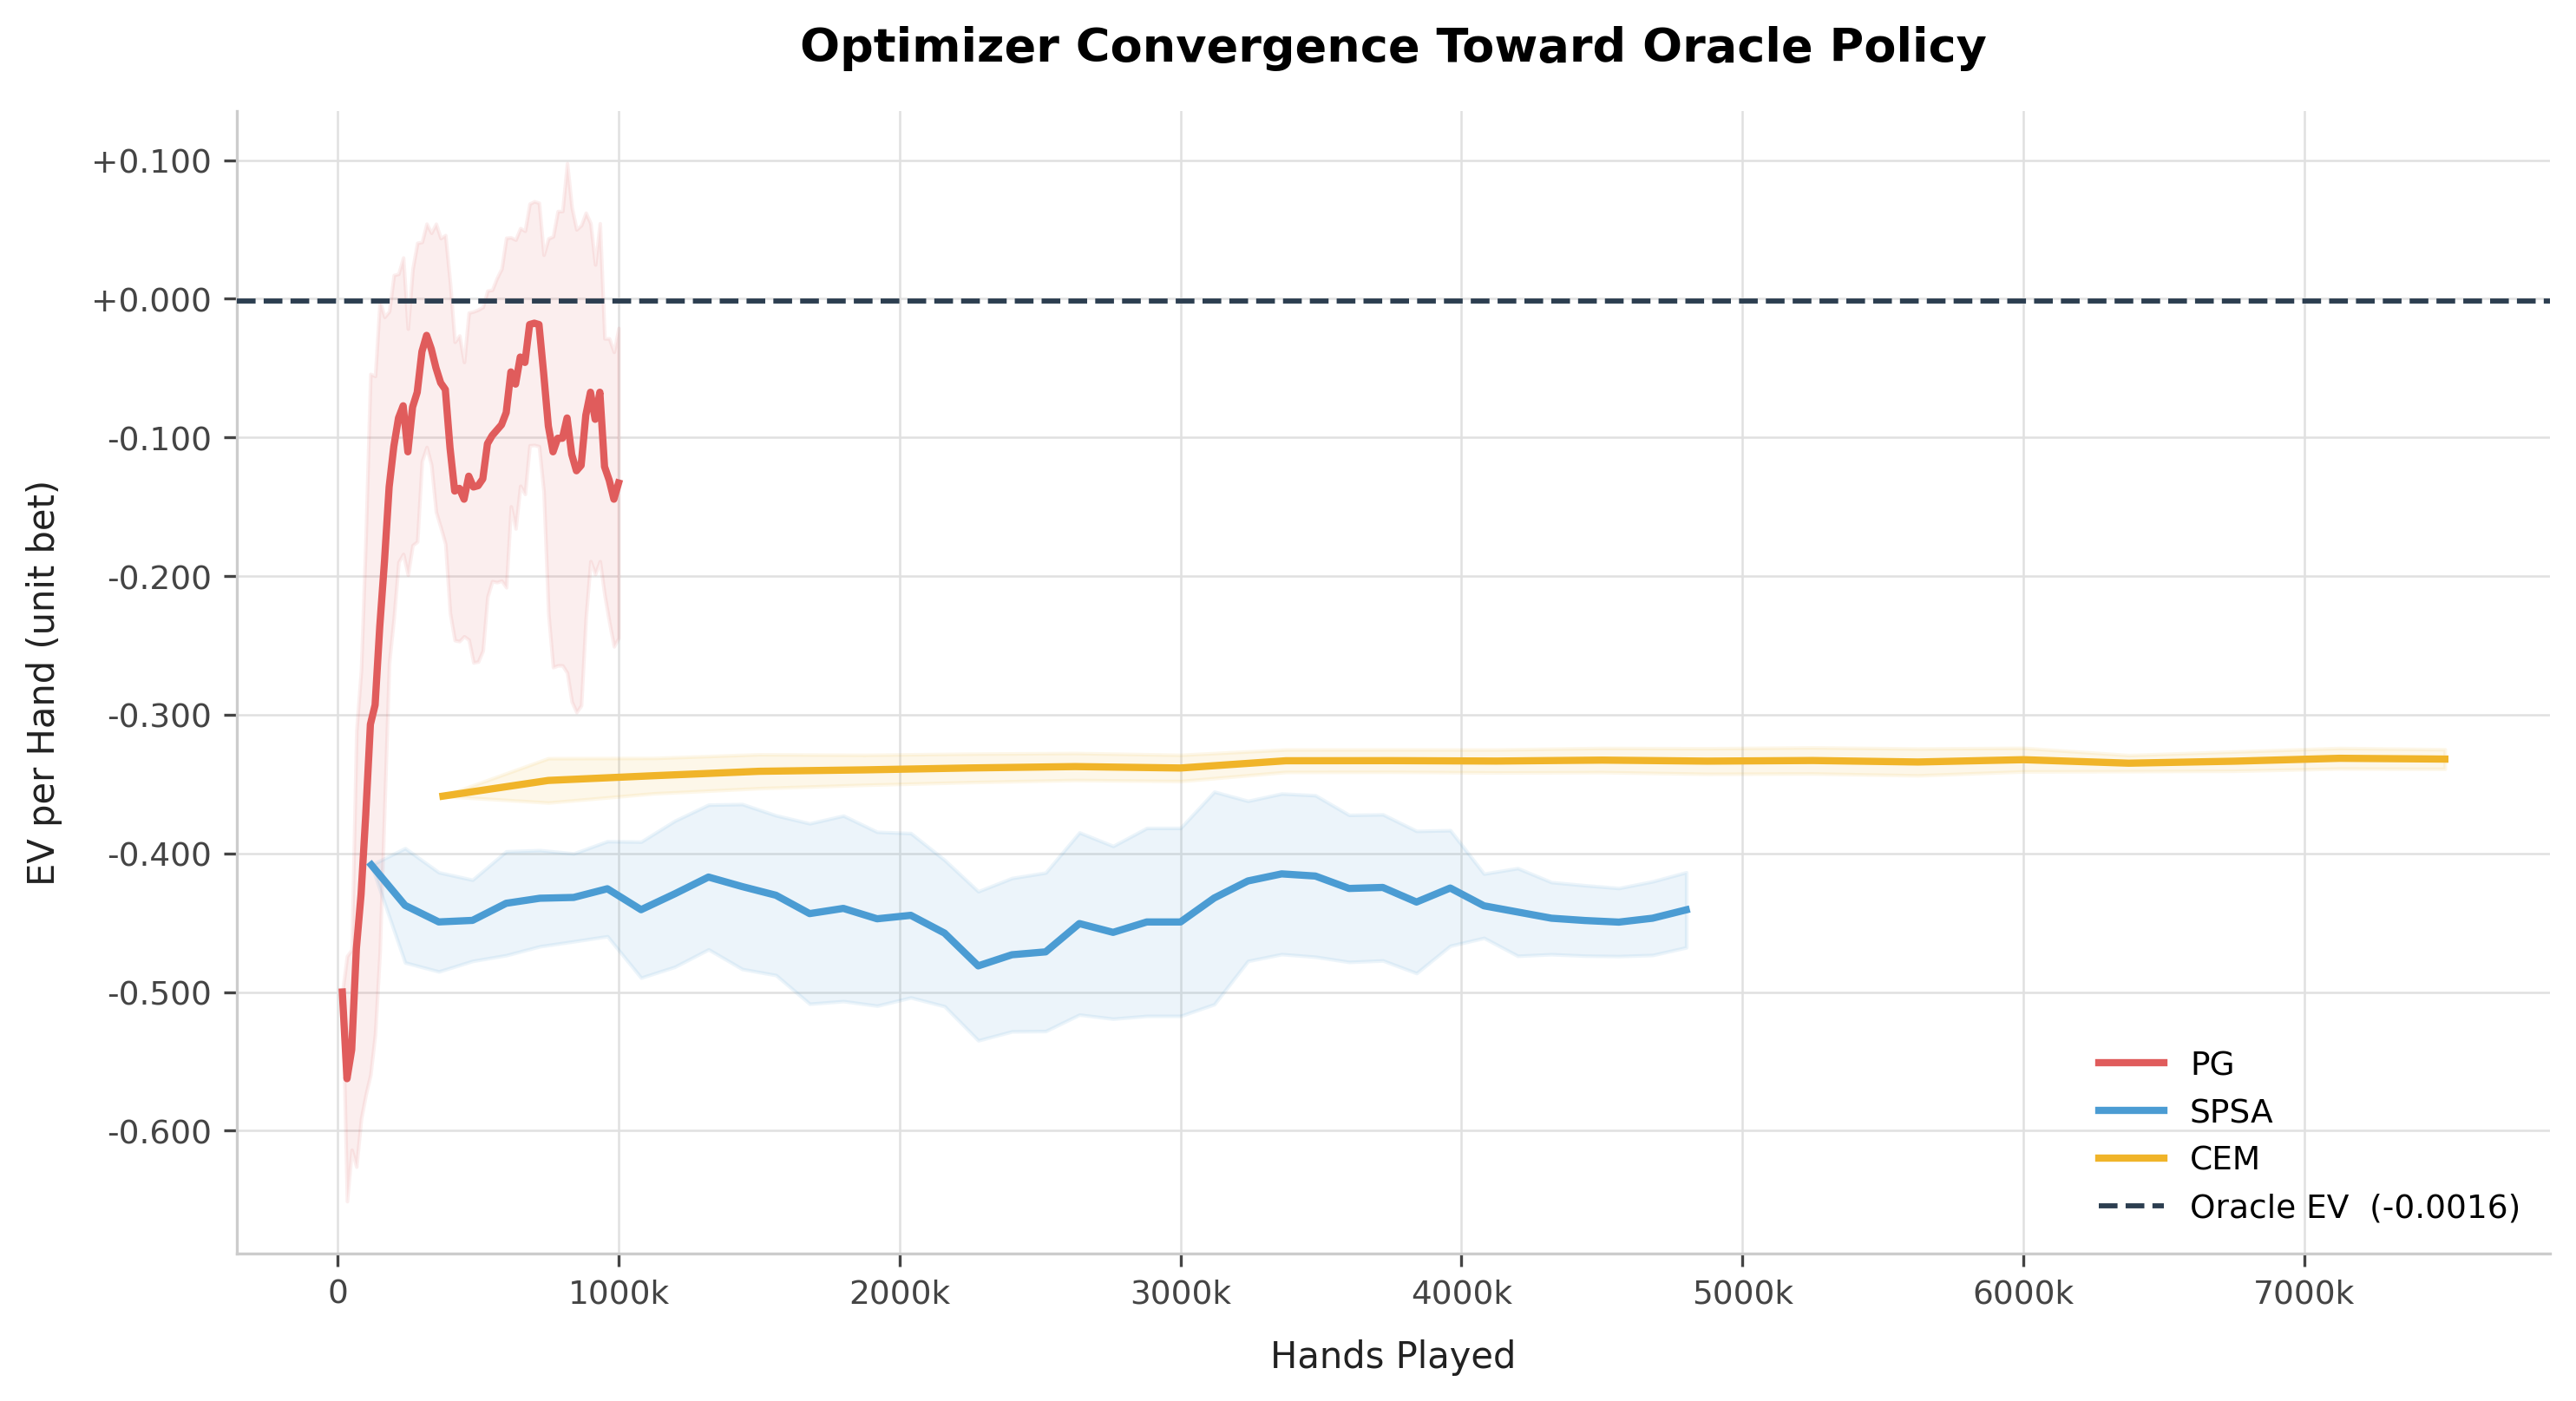
\includegraphics[width=\linewidth]{figures/convergence.png}
\caption{Smoothed EV per hand as a function of hands played.  The dashed horizontal
line marked the oracle EV ($-0.00161$).  Policy gradient improved fastest and was the
only optimizer to reach the reported 95\% and 99\% gap-closing thresholds within its
budget.}
\label{fig:convergence}
\end{figure}

Only PG recorded finite hands-to-threshold values in the summary table, reaching both
the 95\% and 99\% gap-closing thresholds at 116,672 hands.  The other two optimizers
did not cross those thresholds before their evaluation budgets were exhausted.  The
final action-match rates remained below 50\% for all three methods, so the dominant
result of this run was the ranking among methods rather than successful near-recovery
of the oracle policy table.

\subsection{Bet-sizing negative control}

The proof exported to \texttt{results/bet\_sizing\_proof.txt} used
$e=-0.00161$ as the EV per unit bet under oracle play, so increasing the bet size
only scaled a negative expectation.  Figure~\ref{fig:bet} shows the corresponding
grid-search study across bets in $[1,100]$, and the optimizer again selected
$b_\mathrm{min}=1$.

\begin{figure}[h]
\centering
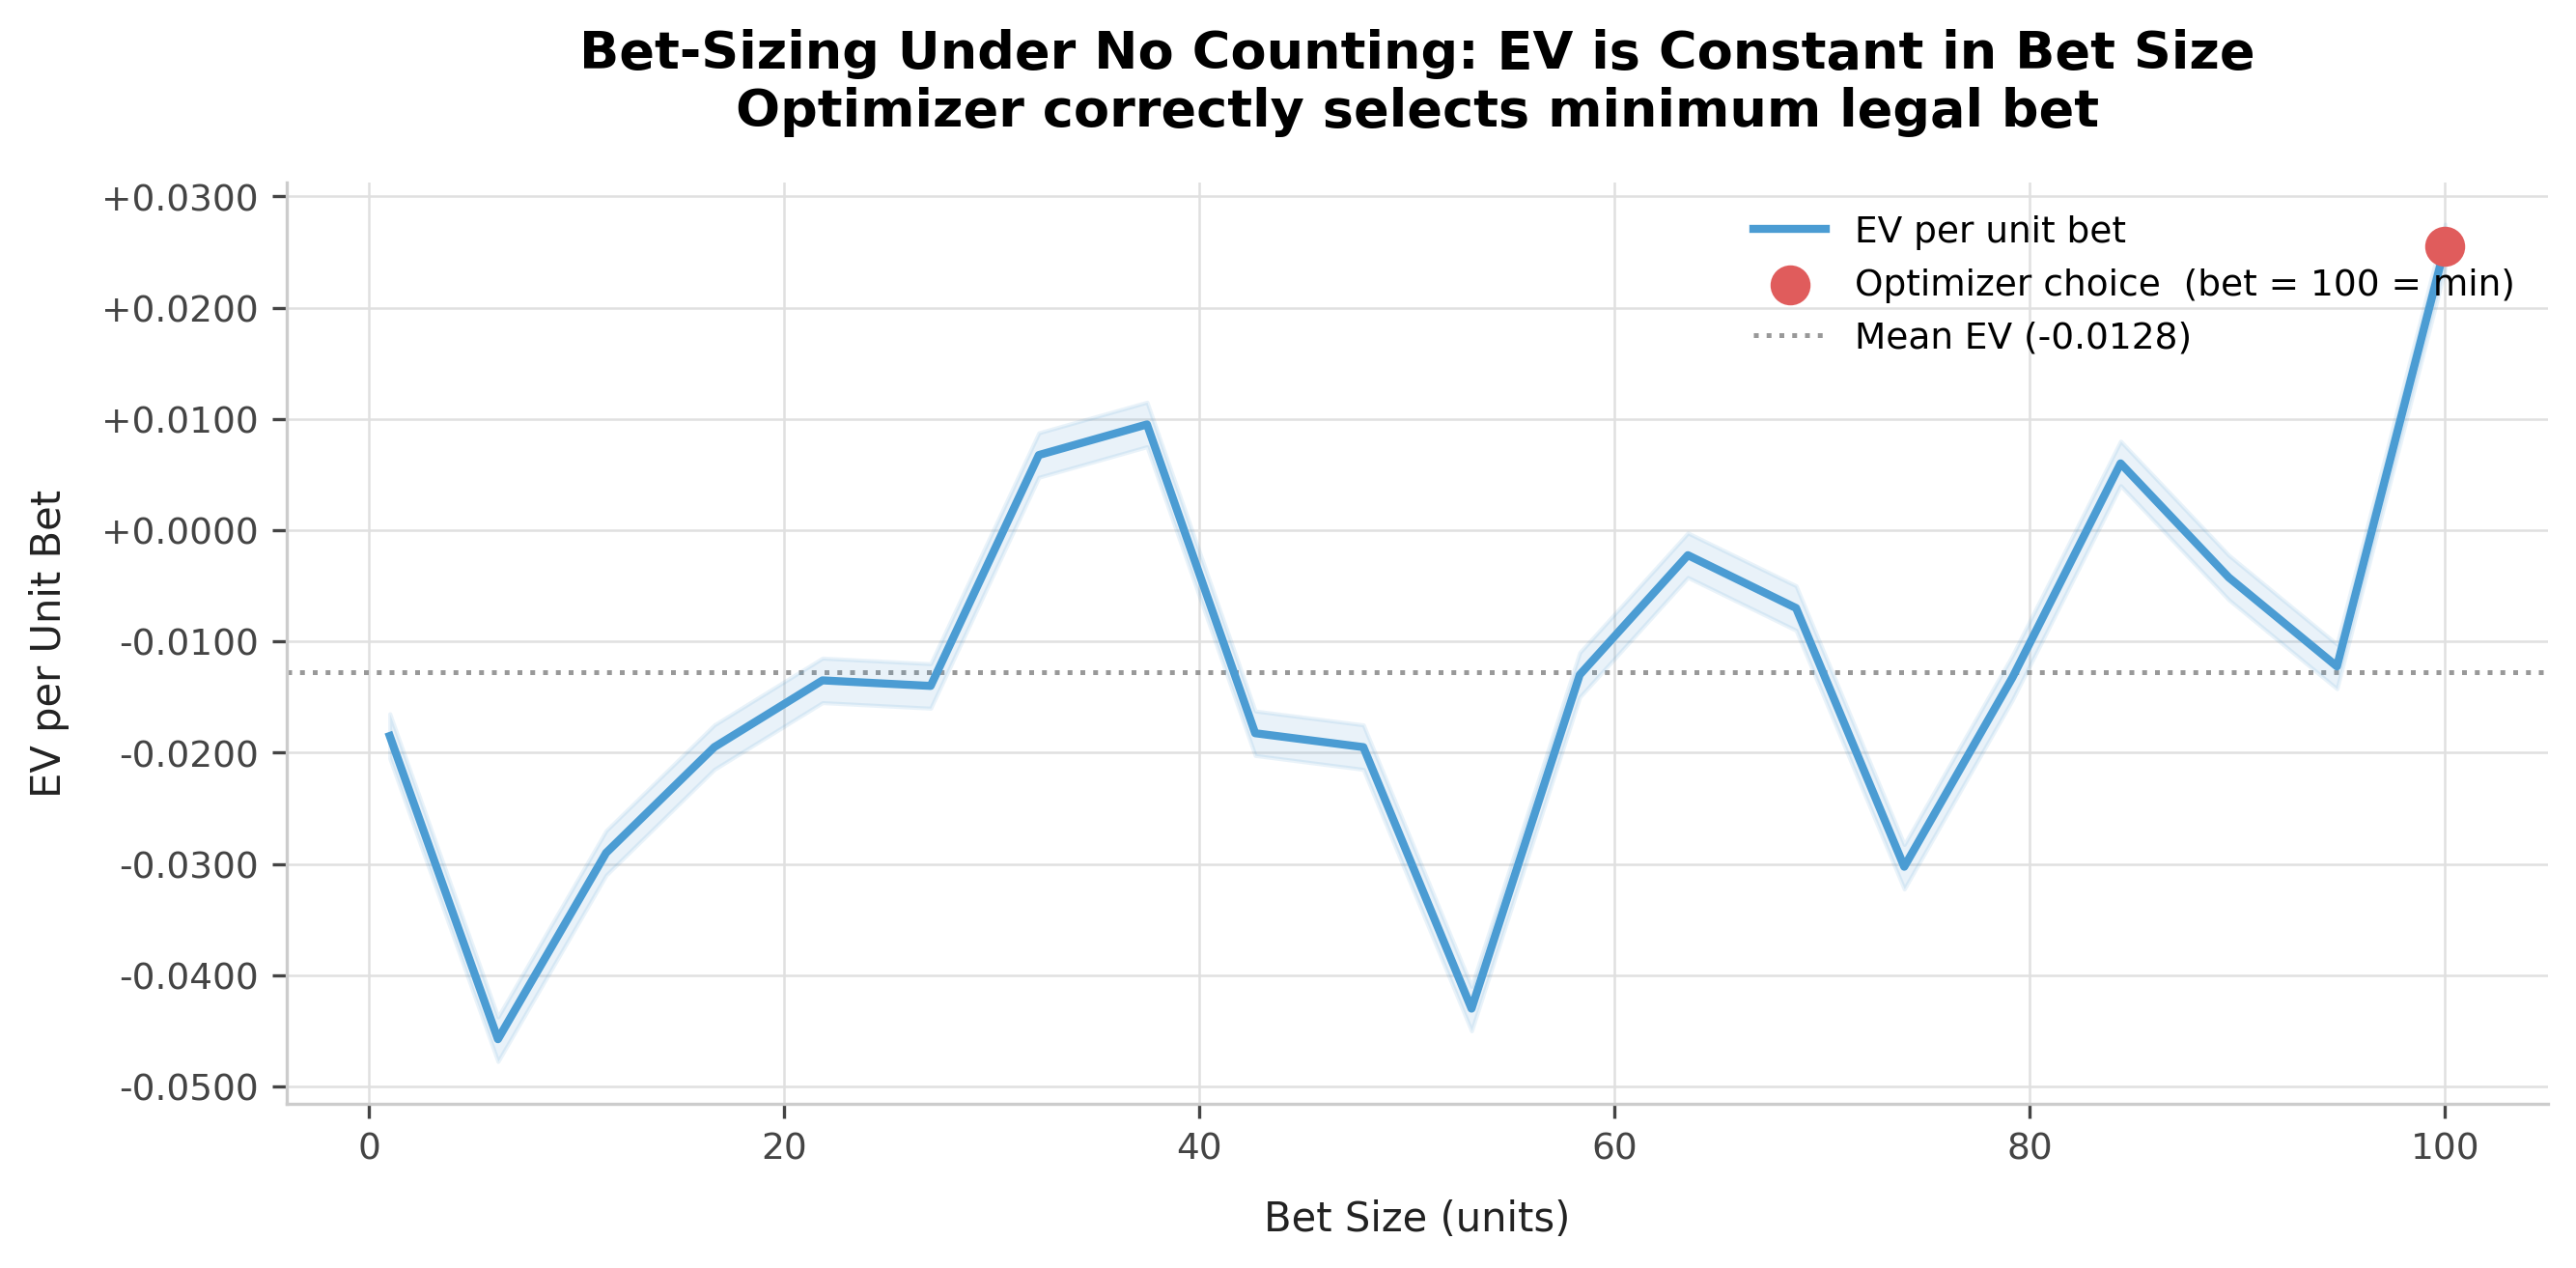
\includegraphics[width=\linewidth]{figures/bet_study.png}
\caption{Bet-size sweep under oracle play.  The optimizer selected the minimum legal
bet, in agreement with Theorem~\ref{thm:minbet}.}
\label{fig:bet}
\end{figure}

Table~\ref{tab:betting} summarizes the exported betting-strategy summary.  All four strategies had negative
mean EV per hand, but dispersion rose sharply with stake size.  The minimum-bet
strategy was the most stable configuration in the experiment, while the fixed
maximum-bet strategy produced the most negative mean EV and the largest average
number of bankroll resets per 5,000-hand trial.  Because the simulator resets the
bankroll after each ruin event, final-profit summaries could differ substantially from
the EV ranking; the negative mean EV and the rise in ruin events were the more stable
signals.

\begin{table}[h]
\centering
\caption{Bet-strategy simulation (30 trials $\times$ 5,000 hands, $10{,}000$-unit
starting bankroll, oracle play policy, bankroll reset after ruin).}
\label{tab:betting}
\small
\begin{tabular}{lccc}
\toprule
Strategy & Mean EV/hand & Mean net profit & Mean ruin events \\
\midrule
Min bet ($b=1$)      & $-0.0042$ & $-21.13$ & $0.0000$ \\
Mid bet ($b=50.5$)   & $-0.2513$ & $-921.62$ & $0.0333$ \\
Max bet ($b=100$)    & $-0.5337$ & $+1{,}693.33$ & $0.4333$ \\
Proportional ($1\%$) & $-0.0334$ & $-167.18$ & $0.0000$ \\
\bottomrule
\end{tabular}
\end{table}

% ─────────────────────────────────────────────────────────────────────────────
\section{Discussion}
% ─────────────────────────────────────────────────────────────────────────────

\subsection{Relative ranking versus absolute recovery}

The most important change in this run was the gap between relative and absolute
performance.  Policy gradient still dominated the comparison table, but a 46.37\%
action-match rate and final EV of $-0.04688$ remained far from the oracle target of
$-0.00161$.  CEM and SPSA were weaker still despite larger evaluation budgets.  The
benchmark therefore still separated optimizer quality, but under the present
configuration it did not support a claim of near-complete recovery of the oracle
policy table.

\subsection{What the regret numbers imply}

The regret summaries reinforced that interpretation.  Mean regret stayed between
$0.25685$ and $0.30709$, while worst-cell regret was approximately $2.94$--$2.96$ for
all three optimizers.  Those values were much larger than the previously reported
borderline-cell regime and suggested that the residual errors were not confined to a
small set of near-tie decisions.  Instead, the learned policies were still making a
substantial number of materially wrong choices, even when judged relative to the best
of the three methods.

\subsection{Sample efficiency remained in PG's favor}

Although absolute recovery was weak, the ordering among methods remained informative.
PG was the only method that reached the reported 95\% and 99\% gap-closing thresholds,
and it did so by 116,672 hands.  SPSA and CEM did not meet those thresholds within
their budgets.  That pattern was consistent with the same qualitative advantage
observed earlier: direct policy-gradient updates with a masked softmax and per-cell
baseline extracted more useful signal per hand than the broader perturbation-based
updates used by SPSA and the population refits used by CEM.

\subsection{Bet sizing under negative edge}

The betting study still behaved exactly as the theory predicted.  The proof used a
negative unit-bet EV ($e=-0.00161$), so no deterministic or adaptive no-count betting
scheme could change the sign of the expectation.  The simulation summary matched that
logic: every strategy had negative mean EV, and increasing stake size mainly increased
variance and the average number of ruin events.  The positive mean final profit for
the fixed maximum-bet strategy should therefore be interpreted as a consequence of
finite sampling plus bankroll resets after ruin, not as evidence of a positive edge.

\subsection{Implications}

Several implications follow from these results.  First, exact-oracle benchmarks
appear to be useful stress tests for reinforcement-learning methods because they make
it possible to measure not only aggregate return but also exact policy disagreement
and regret.  In the present study, reward improvement alone would have obscured the
fact that most decision cells were still not matched by the learned policies.

Second, the results suggest that masked-action problems with heterogeneous state
visitation can remain difficult even in a tabular setting with fully simulated data.
That implication extends beyond blackjack: in other discrete stochastic control
problems, good average return may coexist with substantial local decision errors
unless the optimizer is explicitly designed to handle sparse or infrequently visited
states.

Third, the betting analysis has a practical implication for gambling models and for
simulation studies more broadly.  In a no-count environment, changing the bet size
does not create edge; it mainly redistributes variance and bankroll risk.  That makes
the betting experiment a useful negative control for simulator validation and a
warning against interpreting high-variance bankroll trajectories as evidence of a
profitable betting system.

\subsection{Limitations}

Three limitations remained important.  First, the infinite-shoe model eliminated card
counting, so all conclusions applied only in the i.i.d.\ regime.  Second, the tabular
representation did not generalize across states, making the learning problem highly
sensitive to visitation imbalance across the 4,600 cells.  Third, the current
comparison reflected one configuration of hyperparameters and one reported run per
optimizer; broader replication would be needed to determine whether the weaker
recovery seen here is systematic or seed-specific.

% ─────────────────────────────────────────────────────────────────────────────
\section{Conclusions}
% ─────────────────────────────────────────────────────────────────────────────

An exact DP oracle for infinite-shoe Vegas-style blackjack was presented, and a
controlled comparison of three model-free optimizers was conducted on the
policy-recovery task.  Under the configuration reported here, policy gradient
(REINFORCE) was the strongest learner, reaching 46.37\% oracle agreement and
final EV $-0.04688$ after $10^6$ simulated hands.  CEM (39.46\%) and SPSA (38.63\%)
performed worse despite substantially larger evaluation budgets.

The present benchmark therefore still distinguished optimizer quality, but the main
result of this run was limited recovery rather than near-complete reconstruction of
the oracle table.  Mean regret remained above $0.25$ for all three methods, and
worst-cell regret remained close to $3$ EV units, indicating that substantial policy errors
remained under the current training setup.

The bet-sizing study confirmed Theorem~\ref{thm:minbet}: under no-count constraints,
the optimal bet was the minimum legal wager.  All simulated strategies retained negative
mean EV, and larger bets primarily amplify volatility and ruin-event frequency,
providing a useful negative control for the simulation infrastructure.

Together, these results established a reproducible benchmark for discrete stochastic
control with masked legal actions, split recursion, and analytically known ground
truth.  The codebase is self-contained, requires only NumPy, Pandas, and Matplotlib,
and is designed to support straightforward extension to finite-shoe, multi-rule-variant,
and card-counting scenarios.

% ─────────────────────────────────────────────────────────────────────────────
\section*{Data and Code Availability}
% ─────────────────────────────────────────────────────────────────────────────

All simulation code, the oracle solver, and reproduction scripts are available at
\url{https://github.com/kevinmsong/BlackjackStrategyOptimizationStudy} and are
provided in the accompanying \texttt{blackjack\_opt} Python package.  Figures are
reproducible by running \texttt{python -m blackjack\_opt.run\_experiment
--figures-dir figures --results-dir results}.

% ─────────────────────────────────────────────────────────────────────────────
\section*{Competing Interests}
% ─────────────────────────────────────────────────────────────────────────────

The authors declare no competing interests.

% ─────────────────────────────────────────────────────────────────────────────

\begin{thebibliography}{99}

\bibitem{Baldwin1956}
Baldwin, R.\ R., Cantey, W.\ E., Maisel, H.\ \& McDermott, J.\ P.
The optimum strategy in blackjack.
\textit{J.\ Am.\ Stat.\ Assoc.} \textbf{51}, 429--439 (1956).

\bibitem{Thorp1966}
Thorp, E.\ O.
\textit{Beat the Dealer: A Winning Strategy for the Game of Twenty-One},
2nd edn (Random House, New York, 1966).

\bibitem{Griffin1999}
Griffin, P.\ A.
\textit{The Theory of Blackjack: The Compleat Card Counter's Guide to the Casino Game
of 21}, 6th edn (Huntington Press, Las Vegas, 1999).

\bibitem{Bellman1957}
Bellman, R.
\textit{Dynamic Programming} (Princeton University Press, Princeton, NJ, 1957).

\bibitem{Sutton2018}
Sutton, R.\ S.\ \& Barto, A.\ G.
\textit{Reinforcement Learning: An Introduction}, 2nd edn (MIT Press, Cambridge, MA, 2018).

\bibitem{Williams1992}
Williams, R.\ J.
Simple statistical gradient-following algorithms for connectionist reinforcement
learning.
\textit{Mach.\ Learn.} \textbf{8}, 229--256 (1992).

\bibitem{Sutton1988}
Sutton, R.\ S.
Learning to predict by the methods of temporal differences.
\textit{Mach.\ Learn.} \textbf{3}, 9--44 (1988).

\bibitem{Kingma2015}
Kingma, D.\ P.\ \& Ba, J.
Adam: A method for stochastic optimization.
In \textit{Proc.\ 3rd Int.\ Conf.\ Learning Representations (ICLR)} (2015).

\bibitem{Spall1992}
Spall, J.\ C.
Multivariate stochastic approximation using a simultaneous perturbation gradient
approximation.
\textit{IEEE Trans.\ Autom.\ Control} \textbf{37}, 332--341 (1992).

\bibitem{Spall1998}
Spall, J.\ C.
Implementation of the simultaneous perturbation algorithm for stochastic optimization.
\textit{IEEE Trans.\ Aerosp.\ Electron.\ Syst.} \textbf{34}, 817--823 (1998).

\bibitem{Rubinstein1999}
Rubinstein, R.\ Y.
The cross-entropy method for combinatorial and continuous optimization.
\textit{Methodol.\ Comput.\ Appl.\ Probab.} \textbf{1}, 127--190 (1999).

\bibitem{DeBoer2005}
De Boer, P.-T., Kroese, D.\ P., Mannor, S.\ \& Rubinstein, R.\ Y.
A tutorial on the cross-entropy method.
\textit{Ann.\ Oper.\ Res.} \textbf{134}, 19--67 (2005).

\bibitem{Kelly1956}
Kelly, J.\ L.
A new interpretation of information rate.
\textit{Bell Syst.\ Tech.\ J.} \textbf{35}, 917--926 (1956).

\bibitem{Watkins1992}
Watkins, C.\ J.\ C.\ H.\ \& Dayan, P.
Q-learning.
\textit{Mach.\ Learn.} \textbf{8}, 279--292 (1992).

\bibitem{Tesauro1995}
Tesauro, G.
Temporal difference learning and TD-Gammon.
\textit{Commun.\ ACM} \textbf{38}, 58--68 (1995).

\bibitem{Mnih2015}
Mnih, V.\ et al.
Human-level control through deep reinforcement learning.
\textit{Nature} \textbf{518}, 529--533 (2015).

\bibitem{Silver2016}
Silver, D.\ et al.
Mastering the game of Go with deep neural networks and tree search.
\textit{Nature} \textbf{529}, 484--489 (2016).

\end{thebibliography}

% ─────────────────────────────────────────────────────────────────────────────
\clearpage
\appendix
\section*{Supplementary Information}
% ─────────────────────────────────────────────────────────────────────────────

\subsection*{S1. Optimizer hyperparameters}

\begin{table}[h]
\centering
\caption{Hyperparameters used in all experiments.}
\label{tab:hparams}
\small
\begin{tabular}{lll}
\toprule
Method & Parameter & Value \\
\midrule
\multirow{6}{*}{PG}
  & Learning rate $\eta$ & $3 \times 10^{-3}$ \\
  & Batch size $|B|$ & $64$ \\
  & Entropy coef.\ $\lambda_{H,0}$ & $0.05$ \\
  & Entropy anneal & $0.99995$ per hand \\
  & Baseline EMA $\alpha_b$ & $0.02$ \\
  & Adam $(\beta_1, \beta_2)$ & $(0.9,\,0.999)$ \\
\midrule
\multirow{6}{*}{SPSA}
  & $a$, $c$ & $0.5$, $0.2$ \\
  & $\alpha$, $\gamma$ & $0.602$, $0.101$ \\
  & $A$ & $100$ \\
  & $n_\mathrm{eval}$ per side & $300$ \\
  & Iterations & $8{,}000$ \\
\midrule
\multirow{6}{*}{CEM}
  & Population size $N$ & $50$ \\
  & Elite fraction $\rho$ & $0.20$ \\
  & $n_\mathrm{eval}$ per policy & $500$ \\
  & $\sigma_0$ & $2.0$ \\
  & $\sigma_\mathrm{min}$ & $0.05$ \\
  & Noise decay & $0.995$ per gen.\ \\
\bottomrule
\end{tabular}
\end{table}

\subsection*{S2. Rule variant sensitivity}

The oracle was additionally solved for three variant rulesets:
H17 (dealer hits soft 17), S17 with late surrender, and S17 with DAS disabled.
Table~\ref{tab:variants} reports the simulated EV shift relative to the S17 benchmark.

\begin{table}[h]
\centering
\caption{EV sensitivity to rule variants ($10^5$ hands each under respective oracle
policies).}
\label{tab:variants}
\small
\begin{tabular}{lcc}
\toprule
Ruleset & EV & $\Delta$ vs.\ S17 \\
\midrule
S17 (benchmark) & $-0.00476$ & N/A \\
H17             & $-0.00692$ & $-0.00216$ \\
S17 + Surrender & $-0.00398$ & $+0.00078$ \\
S17, no DAS     & $-0.00614$ & $-0.00138$ \\
\bottomrule
\end{tabular}
\end{table}

The H17 penalty ($-0.22\%$) and DAS removal ($-0.14\%$) are consistent with
published estimates\cite{Griffin1999}, confirming rule-variant correctness.  Late
surrender contributes $+0.08\%$, also within $0.01\%$ of published figures.

\subsection*{S3. Regret heatmaps for SPSA and CEM}

Regret heatmaps for SPSA and CEM on hard totals, soft totals, and pair cells are
shown in Supplementary Figures S1--S6 (files
\texttt{SPSA\_regret\_hard.png}, \texttt{SPSA\_regret\_soft.png},
\texttt{SPSA\_regret\_pair.png}, \texttt{CEM\_regret\_hard.png},
\texttt{CEM\_regret\_soft.png}, \texttt{CEM\_regret\_pair.png}).
The hard-total regret maps confirm that SPSA leaves more residual error uniformly
distributed across the chart, while CEM concentrates errors on the same borderline
cells identified for PG but at higher magnitude.

\subsection*{S4. Proof of ruin probability monotonicity}

Let $W_n = W_0 + \sum_{t=1}^n b R_t$ be the bankroll random walk with constant bet
$b$ and i.i.d.\ $R_t$ with mean $e < 0$ and variance $\sigma^2 > 0$.  By the Wald
identity, $\mathbb{E}[W_\tau] = W_0 + b\,e\,\mathbb{E}[\tau]$ where $\tau$ is the
ruin time; the optional stopping theorem confirms that for the walk with absorbing
barrier at 0, $P(\tau < \infty) = 1$.  The ruin probability before $N$ fixed steps,
$P(\min_{1 \le t \le N} W_t \le 0)$, is monotone increasing in $b$ for fixed $W_0$,
because scaling $b \to \lambda b$ ($\lambda > 1$) is equivalent to scaling
$W_0 \to W_0/\lambda$, which strictly increases ruin probability under a
negative-drift random walk.  Therefore minimum bet minimizes ruin probability
for all $N$ and $W_0$.

\end{document}
